\section{Présentation de Dynamease}

Dynamease est une start up créée par Yves \bsc{Nicolas} en janvier 2014. Le modèle d'affaire de DYNAMEASE est celui d’un éditeur du type \textit{Software As A Service} facturant à ses utilisateurs un abonnement mensuel.

\subsection{L'équipe} 

\subsubsection{Yves Nicolas}

Initiateur du projet Dynamease, son expérience multiple et sa polyvalence sur les sujets techniques, marketing et commerciaux lui ont permis de créer l’entreprise Dynamease, en ayant la vision stratégique, marketing et la mise en œuvre technologique de l’entreprise. Il était mon maître de stage et mon chef de projet.

\subsubsection{Etienne Laplane}

Employé de Dynamease en charge de l’architecture du service Dynamease et du serveur pour les communications téléphoniques : Asterisk.


\section{Présentation du service Dynamease}

\subsection{Les objectifs}

Dynamease se base sur le fait que le portable est un appareil téléphonique qui devient plus utilisé que les téléphones fixes. Le portable devient, grâce à Dynamease, un standard automatisé. Tous les appels entrant sont filtrés en amont afin de déterminer leur importance et leur provenance. Il est possible pour un utilisateur Dynamease de configurer les services Dynamease afin de déterminer des horaires d'appel pour différents types de contact (Professionnel, Familial, ami). Une fois les appels filtrés, ils sont redirigés vers l'appareil téléphonique de l'utilisateur.

Lors du filtrage, des informations sont récupérées sur les appels entrants. Ces informations sont récupérées sur les bases de données privées du client ainsi que sur des bases de données publiques (Annuaire inverse, réseaux sociaux ...). Les appels redirigés sont alors accompagnés par ces informations. Les informations pertinentes, sur l'appel, sont affichées sur l'appareil téléphonique de l'utilisateur.\\

Ce service permet aux utilisateurs de déléguer la partie standardisation de leur entreprise et d'éviter de rater des appels importants tout en ignorant les appels pouvant être considérés comme nuisibles. De plus Dynamease propose aux entreprises de diminuer leurs coûts de téléphonie en remplaçant les appareils fixes de l'entreprise par les téléphones portables de leurs employés. Les employés pourront ainsi avoir un seul appareil téléphonique pour leurs appels, et configurer leurs horaires d'appel professionnel en fonction de leurs horaires de travail.\\

L'entreprise Dynamease est également soucieuse des adolescents sortis du système scolaire. Dynamease veut proposer une aide à ses "décrocheurs" en les formant sur le métier de l'informatique, en leur faisant réaliser, sur une période courte, des petits projets. L'initiative, "de décrocheur à développeur" verra le jour durant mon stage.

\subsection{Les différentes offres}

Dynamease propose à ses clients plusieurs offres. Chaque offre contient des fonctionnalités particulières ainsi que les fonctionnalités des offres précédentes dans la hiérarchie.  La hiérarchie des offres ainsi que les fonctionnalités attribuées à chacune de ces offres est indiquée dans le diagramme suivant:

\begin{figure}[!h]
	\centering
	\includegraphics[scale=0.5]{img/useCase.png}
	\caption{\label{useCase} Diagramme des cas d'utilisation Dynamease}
\end{figure}

Nous allons maintenant décrire ces différentes offres.

\subsubsection{Basic}

L'offre \textit{Basic} est une offre gratuite, permettant à l'utilisateur d'accéder aux fonctions basiques de l'application téléphonique et de l'application web:

\begin{itemize}
	\item Envoi de cartes de visite Dynamease;
	\item Gestion de la liste de contact;
	\item Gestion manuelle de la disponibilité.
\end{itemize}

\subsubsection{Avantage}

L'offre Avantage s'adresse aux clients particuliers, désirant avoir une gestion de leur disponibilité gérée par rapport à des calendriers (Calendrier Dynamease ou \textit{Google Calendar}).

\subsubsection{Privilège}

L'offre Privilège permet aux utilisateurs d'acquérir un numéro Dynamease. Ce numéro permet à l'utilisateur d'être joint sur n'importe lequel de ses appareils téléphoniques. Les appels entrant en direction de ce numéro sont gérés par le serveur Dynamease. Celui-ci identifiera l'appel, définira son importance et enfin le redirigera vers l'appareil téléphonique de l'utilisateur.

\subsubsection{Intégrale}

L'offre Intégrale est destinée aux entreprises. Cette offre permet l'ajout d'employés qui auront les mêmes fonctionnalités qu'un client  Avantage.

Il est également possible d'ajouter des connecteurs. Les connecteurs permettent une meilleure identification d'appel ainsi qu'une meilleure redirection. Les connecteurs sont des bases de données fournies par les entreprises qui permettent d'identifier un appelant ainsi que la redirection vers l'employé responsable de celui-ci. Les connecteurs sont utilisés pour fournir des informations sur l'appelant et également pour leur redirection.

\section{Présentation de l'environnement Dynamease}

\subsection{Environnement du service Dynamease}

Nous allons maintenant présenter l'environnement Dynamease. Dynamease suit le pattern MVC (Modèle View Controler). On peut représenter l'environnement principal de Dynamease avec le diagramme suivant.

\newpage

\begin{figure}[!h]
	\centering
	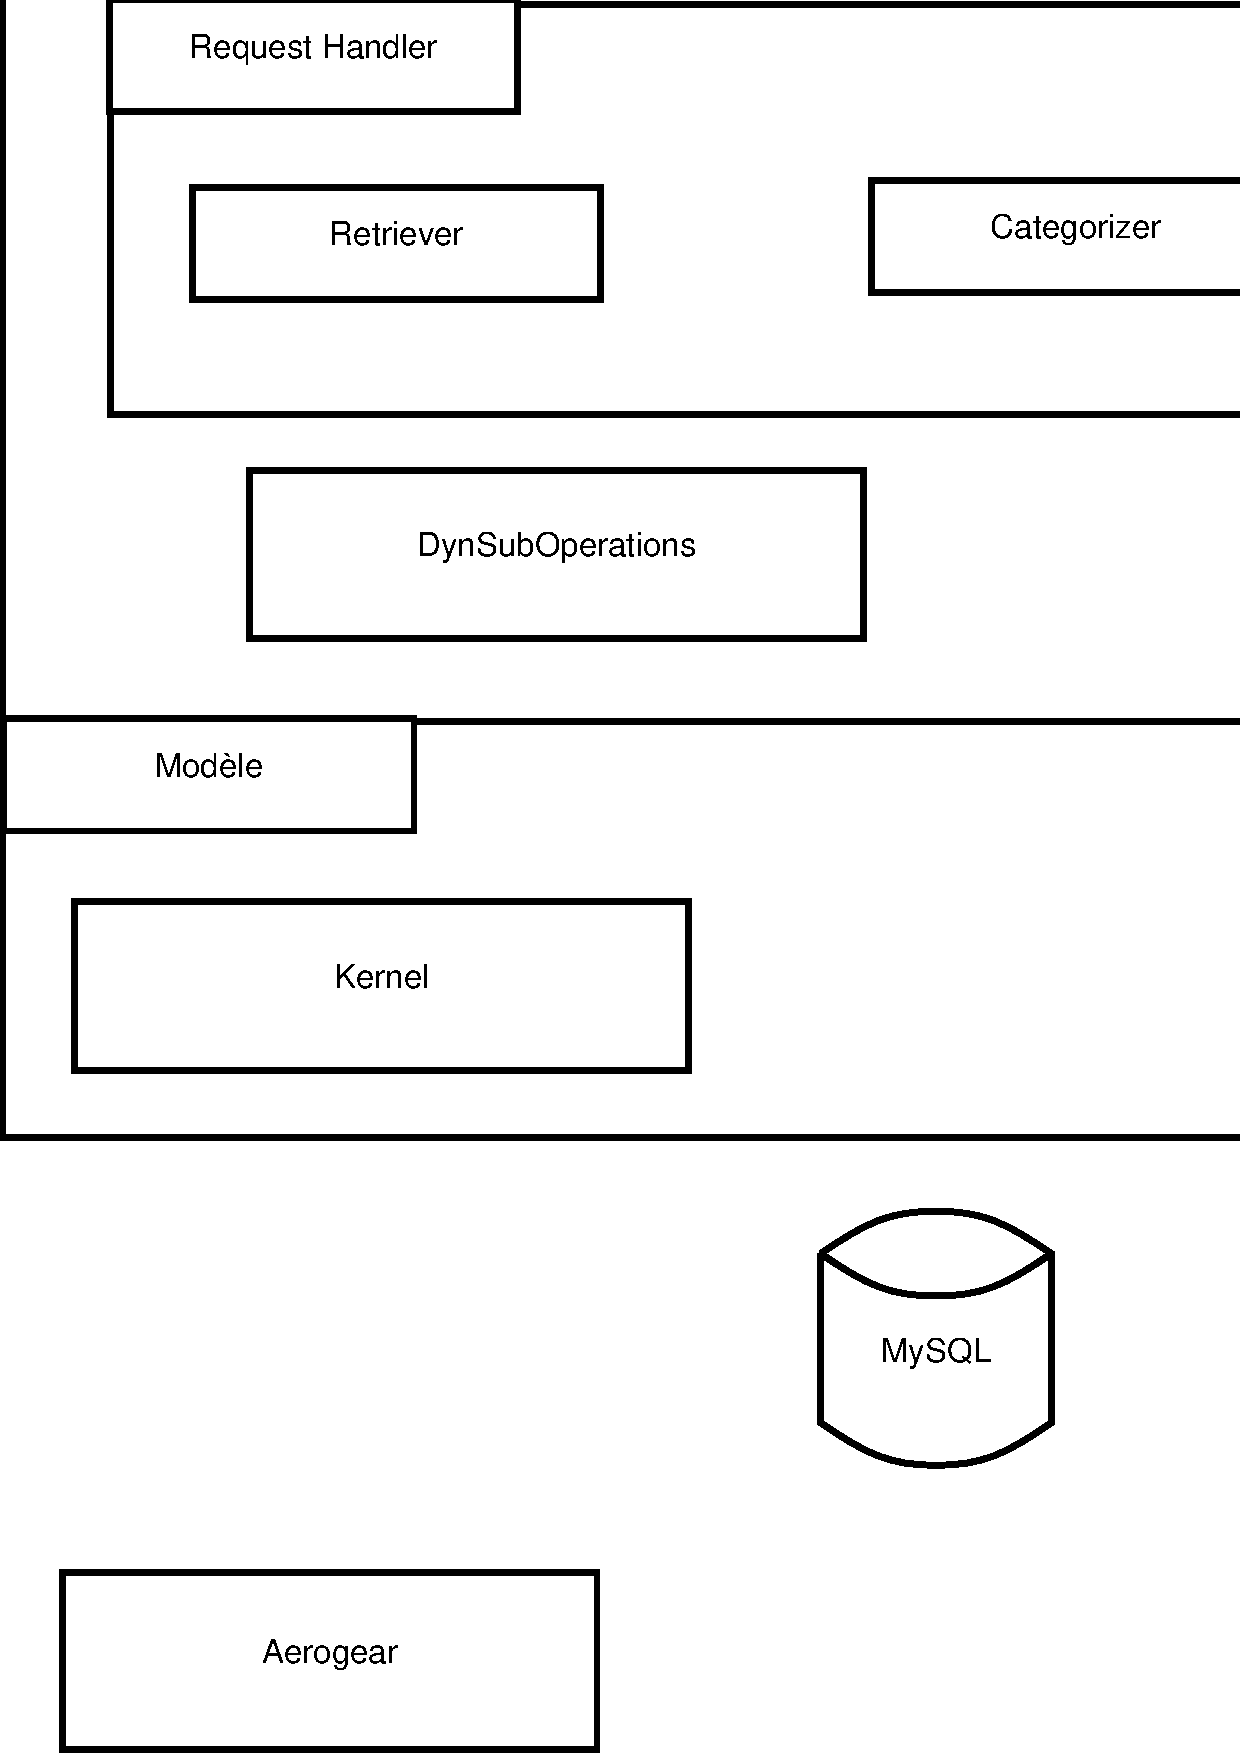
\includegraphics[scale=0.4]{img/composant.pdf}
	\caption{\label{composant} Les différents composants de l'environnement Dynamease}
\end{figure}

Présentons ce diagramme du haut vers le bas. Nous avons en haut les applications clientes utilisant les services Dynamease. Ces applications sont la partie web, accessible pour l'utilisateur depuis un navigateur et les applications téléphoniques constituées par les applications Android et Ios.\\

Les services Dynamease sont accessibles via les interfaces de requêtes représentées par JsonRq et Appless par le protocole HTTP. JsonRq réuni toutes les requêtes du type JsonRPC et Appless réuni toutes les requêtes REST. Dynamease dispose de ces deux interfaces car une migration est en cour, toutes les requêtes REST seront transformées en des requêtes JsonRPC.\\

Passons maintenant à la partie Contrôleur. Cette partie peut être divisée en deux composants.

Le premier de ces composants est le RequestHandler, qui s'occupe du traitement des appels. RequestHandler dispose de trois parties. La première partie est le \textit{Retriever}, qui représente la recherche du contact lors d'un appel. Le \textit{Categorizer} réunie toutes les classes aidant à la classification de l'appelant. Et enfin le \textit{Matcher}, a pour rôle de mettre en relation l'appelant avec la meilleure personne à contacter, par le biais du meilleur appareil téléphonique à utiliser pour cette personne.

La seconde partie du Contrôleur réunit toutes les méthodes relatives aux clients, création, suppression, modification et lecture des informations. Les deux classes utilisées dans cette partie sont le CorpSubOperations pour les entreprises, donc du type Intégral. Les autres clients sont gérés par la classe DynSubOperations\\

La partie Modèle de Dynamease est représentée par les parties Core et Kernel. Core représente les classes métier utilisées uniquement par le serveur Dynamease. Quant à la partie Kernel elle réunit toutes les classes pouvant être utilisées par chacune des applications de Dynamease.\\

Le stockage est géré par deux bases de données MySQL et Ldap. La base de données Ldap est utilisée pour stocker les informations sur les contacts des utilisateurs. La base MySQL stocke toutes les autres informations utiles.

La raison de la présence de deux bases de données est dû au fait de répondre à un besoin des futurs clients ayant déjà un annuaire Ldap, afin de faciliter l'importation de leurs contacts.\\

En plus du serveur Dynamease, l'entreprise dispose aussi d'un serveur Asterisk. C'est un serveur gérant les communications téléphoniques. Ce serveur communique avec le serveur Dynamease afin de gérer les redirections et avoir les numéros entrant.\\

Un serveur Aerogear est également présent pour la gestion des notifications Push. Une présentation détaillée de ce serveur sera effectuée dans la suite de ce rapport.

\subsection{Méthode de travail de Dynamease}

La gestion du projet suivait une version modifiée de la méthode Scrum. Le travail n'est pas divisé en Sprint, les fonctionnalités attendues sont données au fur et à mesure. Je n'ai pas trouvé cette méthode adaptée à mon travail. Il était beaucoup plus compliqué d'estimer le temps de chaque tâche en raison de l'absence de \textit{deadline}. De plus ne pas avoir une liste de fonctionnalités à accomplir m'a obligé à être dépendant de mon chef de projet.\\

Le code source des applications Dynamease est sauvegardé sur un dépôt Git. Il nous permet de garder une version de chacun de nos codes sources. Son système de branche est très utile en particulier pour pouvoir revenir plus rapidement à une version de production de l'application.